% Created 2024-07-23 Tue 11:41
% Intended LaTeX compiler: pdflatex
\documentclass[10pt]{article}
% =================================BASE====================================%
\usepackage[left=2cm,right=2cm,top=2cm,bottom=2cm]{geometry} % Marges
\usepackage[T1]{fontenc} % Nécessaire avec FrenchBabel
\usepackage[utf8]{inputenc} % Important pour symboles Francophones, é,à,etc
\usepackage{csquotes} % Recommandé par PDFLatex lors de la compilation. 

% Calligraphie
%\usepackage{pxfonts} % Met le texte ET les maths en Palatino + donne accès à des symboles math
\usepackage{palatino} % Cette commande met seulement le texte en police palatino
\usepackage{lmodern} % Pour les maths? Lmodern pour les maths
% Use lmodern for sans-serif
\usepackage{mathrsfs} % Permet la command \mathscr (Lettres attachées genre) \mathscr(B)

% Bibliographie
%\usepackage[backend=bibtex,style=phys,sorting=ynt]{biblatex}
\usepackage[backend=biber,sorting=ynt,style=authoryear]{biblatex} % N'est pas utilisé par le compilateur org-mode, mais NÉCESSAIRE. Voir le fichier init.el pour changer le style. 
\addbibresource{/home/charlesedouard/Desktop/Travail/Documentation/2023/master-bibliography.bib}


\usepackage{amsmath, amssymb, amsthm} % Symb. math. (Mathmode+Textmode) + Beaux théorèmes.
\usepackage{mathtools,cancel,xfrac} % Utilisation de boîtes \boxed{} + \cancelto{}{}, xfrac
\usepackage{graphicx, wrapfig} % Géstion des figures.
\usepackage{hyperref} % Permettre l'utilisation d'hyperliens.
\usepackage{color} % Permettre l'utilisation des couleurs.
\usepackage{colortbl} % Color tables
\usepackage[dvipsnames]{xcolor} % Couleurs avancées.

% Physique
\usepackage{physics} % Meilleur package pour physicien. 

% Style
\usepackage{lipsum} % For fun
\usepackage{tikz} % Realisation de figures TIKZ.
\usetikzlibrary{arrows.meta,bending} % Arrow heads 
\usepackage{empheq} % Boite autour de MULTIPLE équations
\usepackage{bbding}

% Français
\usepackage[french]{babel} % Environnements en Français.

\usepackage{titling} % Donne accès à \theauthor, \thetitle, \thedate

% ==============================BASE-(END)=================================%





% ================================SETTINGS=================================%
% Pas d'indentation en début de paragraphe :
\setlength\parindent{0pt}
\setlength{\parskip}{0.15cm}

% Tableaux/tabular
% Espace vertical dans les tabular/tableaux
\renewcommand{\arraystretch}{1.2}
% Couleur des tableaux/tabular
% \rowcolors{3}{violet!5}{}

% Couleurs de hyperliens :
\definecolor{mypink}{RGB}{147, 0, 255}
\hypersetup{colorlinks, 
             filecolor=mypink,
             urlcolor=Violet, 
             citecolor=mypink, 
             linkcolor=mypink, 
             anchorcolor=mypink}


% Numéros d'équations suivent les sections :
\numberwithin{equation}{section} 

% Les « captions » sont en italique et largeur limitée
\usepackage[textfont = it]{caption} 
\captionsetup[wrapfigure]{margin=0.5cm}

% Retirer l'écriture en gras dans la table des matières
\usepackage{tocloft}
\renewcommand{\cftsecfont}{\normalfont}
\renewcommand{\cftsecpagefont}{\normalfont}

% Change bullet style
\usepackage{pifont}
\usepackage{enumitem}
%\setlist[itemize,1]{label=\ding{224}}
\setlist[itemize,1]{label=\ding{239}}
\renewcommand{\boxtimes}{\blacksquare}
% ================================SETTINGS=================================%



% ==============================NEWCOMMANDS================================%
% CQFD symbol
\renewcommand{\qedsymbol}{$\hfill\blacksquare$}

% Vecteurs de base :
\newcommand{\nvf}{\vb{\hat{n}}}
\newcommand{\evf}{\vb{\hat{e}}}
\newcommand{\ivf}{\vb{\hat{i}}}
\newcommand{\jvf}{\vb{\hat{j}}}
\newcommand{\kvf}{\vb{\hat{k}}}
\newcommand{\uu}{\vb{u}}
\newcommand{\vv}{\vb{v}}
\newcommand{\ust}{\vb{u}_{\ast}}

% Physics empty spaces 
\newcommand{\short}{\vphantom{pA}}
\newcommand{\tall}{\vphantom{pA^{x^x}_p}}
\newcommand{\grande}{\vphantom{\frac{1}{xx}}}
\newcommand{\venti}{\vphantom{\sum_x^x}}
\newcommand{\pt}{\hspace{1pt}} % One horizontal pt space

% Moyenne numérique entre deux points de grilles. 
\newcommand{\xmean}[1]{\overline{#1}^x}
\newcommand{\ymean}[1]{\overline{#1}^y}
\newcommand{\zmean}[1]{\overline{#1}^z}
\newcommand{\xymean}[1]{\overline{#1}^{xy}}

% Tilde over psi
\newcommand{\tpsi}{\tilde{\psi}}
\newcommand{\tphi}{\tilde{\phi}}

% Nota Bene env : (\ding{89})
%\newcommand{\nb}{$\boxed{\text{\footnotesize\EightStarConvex}\pt \mathfrak{N. B.}}$\hspace{4pt}}
\newcommand{\nb}{\underline{{\footnotesize\EightStarConvex}\pt $\mathfrak{N.B.}$\vphantom{p}}\hspace{3pt}}

\newcommand{\exemple}{
\parbox[center]{2.2cm}{\begin{tcolorbox}[sharp corners, rounded corners=northeast, rounded corners=southeast,
colback=Violet!5, colframe=black,
size=small, width=2cm, left=-0.25pt, bottom=-0.5pt,
arc is angular, arc=2.5mm, boxrule=0.35pt, leftrule=4pt, %bottomrule=1pt,
after={\enskip}] Exemple \end{tcolorbox}}}

\newcommand{\cqfd}{\hfill$\blacktriangleleft$}

% Define the nota bene environment
\usepackage{tcolorbox}
\newtcolorbox{notabene}{
     colback=blue!5,
     colframe=black,
     boxrule=0.5pt,
     arc=2pt,
     left=5pt,
     right=5pt,
     top=5pt,
     bottom=5pt,
}


\newcommand{\cmark}{\ding{52}}
\newcommand{\xmark}{\ding{55}}
% ==============================NEWCOMMANDS================================%



% ==============================PAGE-TITRE=================================%
% Titlepage 
\newcommand{\mytitlepage}{
\begin{titlepage}
\begin{center}
{\Huge \thesubtitle \par}
\vspace{2cm}
{\Huge \MakeUppercase{\thetitle} \par}
\vspace{2cm}
RÉALISÉ DANS LE CADRE\\ D'UN PROJET POUR \par
\vspace{2cm}
{\Huge ISMER--UQAR \par}
\vspace{2cm}
{\thedate}
\end{center}
\vfill
Rédaction \\
{\theauthor}\\
\url{charles-edouard.lizotte@uqar.ca}\\
ISMER-UQAR\\
Police d'écriture : \textbf{CMU Serif Roman}
\end{titlepage}
}
% ==============================PAGE-TITRE=================================%



% =================================ENTÊTE==================================%
\usepackage{fancyhdr}
\pagestyle{fancy}
\setlength{\headheight}{13pt}
\renewcommand{\headrulewidth}{0.025pt} % Ligne horizontale en haut

\fancyhead[R]{\textit{\thetitle}}
\fancyhead[L]{\ \thepage}
\fancyfoot[R]{\textit{\theauthor}}
\fancyfoot[L]{}
\fancyfoot[C]{} 
% =================================ENTÊTE==================================%
\author{Charles-Édouard Lizotte}
\date{18/08/2023}
\title{Carnet de bord, Université McGill}
\newcommand{\thesubtitle}{Contrat Été 2023}
\hypersetup{
 pdfauthor={Charles-Édouard Lizotte},
 pdftitle={Carnet de bord, Université McGill},
 pdfkeywords={},
 pdfsubject={},
 pdfcreator={Emacs 27.1 (Org mode 9.6.7)}, 
 pdflang={French}}
\begin{document}

\mytitlepage
\tableofcontents\newpage

\section{Reconnection au réseau de McGill -- \textit{<2023-08-14 Mon>}}
\label{sec:org6de5c0b}
Un petit rappel dans mes notes personnelles que mes coordonnées de McGill sont
\begin{verbatim}
  >>> charles-edouard.lizotte@mcgill.ca
\end{verbatim}
et que mon \emph{mot de passe} est exactement le même que mon \emph{mot de passe} professionnel de l'UQAR.
Comme j'utilise mes adresses professionnelle et étudiante de l'UQAR, j'ai rarement besoin d'utiliser celle de McGill.
Donc, ça serait bien qu'elle soit écrite quelque part dans mon carnet de travail si je ne veux pas la perdre.


\section{Problème avec la méthode Leapfrog -- \textit{<2023-08-14 Mon>}}
\label{sec:org1fb7cd8}

\subsection{Nouveau schéma d'intégration leapfrog pour la correction de psi barotrope}
\label{sec:orgb823847}
Pour clarifier la méthode \emph{leapfrog}, la procédure consiste à prendre le champ précédent (à \(t-\delta t\)) et lui additionner le double du \emph{RHS} (pris au temps \(t\)) dans le but d'obtenir le champ au temps \(t+\delta t\).
Conséquemment, la méthode se déclare comme suit, soit
\begin{equation}
   u^{t+\delta t} = u^{t-\delta t} + 2\Delta t\cdot RHS^t.
\end{equation}
Il faut impérativement trouver un moyen d'appliquer cette même méthode dans la correction de MUDPACK.
Si l'on sépare les champs, il est possible qu'on se mélange avec le \(\delta \psi\) comme il y a deux \(\Delta t\) dans la méthode \emph{leapfrog}.\bigskip

Construisons nous une suite d'étapes logiques pour appliquer la méthode \emph{leapfrog} avec MUDPACK.
\begin{enumerate}
\item On calcule \(\delta \psi\) à l'aide de la différence de \(\zeta_{BT}\) entre \(t-\delta t\) et \(t+\delta t\) (voir équation \ref{eq:orgd95a07b}) ;
\item Trouver le \(\psi^{t+\delta t}\) à l'aide de \(\psi^{t-\delta t}\), ce qui se traduit par l'utilisation de MUDPACK pour trouver \(\delta \psi\) (voir équation \ref{eq:org93226c2});
\item Appliquer le filtre de Robert (section \ref{orge2ea21a})  sur les deux quantités (\(\zeta_{BT}\) et \(\psi_{BT}\));
\item Et redéfinir \(\psi^t = \psi^{t+\delta t}\) pour le prochain time step de MUDPACK, de manière identique à ce qu'on fait dans la routine \emph{main.f90}.
\end{enumerate}

Concrétement, on se définit une méthode \emph{leapfrog} pour la correction à l'aide de MUDPACK, soit des champs à trois \emph{étages}, comme dans la fonction \emph{main.f90}.
Nous aurions 3 quantités, soient \(\psi^{t+\delta t}\), \(\psi^t\), \(\psi^{t-\delta t}\) et le \(\delta \psi\) calculé par MUDPACK serait définit par
\begin{equation}
\label{eq:org93226c2}
   \delta \psi = \psi^{t+\delta t} - \psi^{t-\delta t},
\end{equation}
ce qui mettra la condition sur \(\zeta_{BT}\) que
\begin{equation}
\label{eq:orgd95a07b}
   \delta \zeta_{BT} = \zeta_{BT}^{t+\delta t} - \zeta_{BT}^{t-\delta t}.
\end{equation}

\subsection{Filtre de Robert}
\label{sec:org42a579f}
\label{orge2ea21a}
L'application du filtre de Robert est caractérisée par le système d'équations,
\begin{align}
   &\psi^t \ \pt= \psi^t \ + R_f\pt\pt \qty( \psi^{t+\delta t}  +\psi^{t-\delta t} - 2\psi^t)\pt,\\
   &\zeta_{BT}^t = \zeta_{BT}^t + R_f\pt \qty( \zeta_{BT}^{t+\delta t}  +\zeta_{BT}^{t-\delta t} - 2\zeta_{BT}^t),
\end{align}
où \(R_f \sim 0.001\).



\section{Retour au débuggage de MUDPACK -- \textit{<2023-08-15 Tue>}}
\label{sec:orga08ccf6}
Certains indices me permettent de remarquer que le problème pourrait être apparent à l'intérieur de la méthode de relaxation de MUDPACK.
En gros, on a toujours un courant nul au milieu vertical du modèle, ce qui est douteux, mais qui pourrait être un artefact de la méthode employée par MUDPACK lors de sa relaxation.
J'essaye donc d'autre schémas d'intégration, tel que la relaxation par lignes verticales, par exemple.
Mais sinon, je suis assez désespéré\ldots{}

\subsection{État des choses -- \textit{<2023-08-18 Fri>}}
\label{sec:org547f175}

Le nouveau problème apparaît autour de 2 ou 3 jours, comme on peut le voir sur la figure \ref{fig:org2384351}.
Le problème initial de la divergence semble réglé, mais le focus de l'accumulation d'erreur numérique semble s'orienter vers le rotationnel du courant barotrope (\(\boldsymbol{\zeta}_{BT}\)).
Les paramètres de l'expérience sont illustrés au tableau \ref{tab:orge6d199e}.
Après plusieurs jours, une circulation de type Stommel apparraît, mais avec des cercles concentriques qui sont du à l'erreur appliquée par MUDPACK (Voir figure \ref{fig:orge213f4e}).

\begin{table}[htbp]
\caption{\label{tab:orge6d199e}Paramètres de l'expérience réalisée.}
\centering
\begin{tabular}{llrl}
\hline
\hline
Paramètres & Symbole & Valeur & Unité\\[0pt]
\hline
Taille du domaine & L\textsubscript{x} = L\textsubscript{y} & 2000 & km\\[0pt]
Nombre de points de grilles & nx = ny & 513 & --\\[0pt]
Pas de temps & \(\Delta\) t & 300 & s\\[0pt]
Paramètre de Coriolis & f & 7\texttimes{}10\textsuperscript{-5} & s\textsuperscript{-1}\\[0pt]
Paramètre beta & beta & 1\texttimes{}10\textsuperscript{-11} & m\textsuperscript{-1}s\textsuperscript{-1}\\[0pt]
Amplitude du vent & \(\tau\)\textsubscript{atm} & 0.1 & N m\textsuperscript{-2}\\[0pt]
Coefficient de visc. biharmonique & A\textsubscript{bh} & dx\textsuperscript{4} \texttimes{}10\textsuperscript{-5} & s\textsuperscript{-1}\\[0pt]
Coefficient de frottement & r\textsubscript{drag} & 10\textsuperscript{-7} & s\textsuperscript{-1}\\[0pt]
Vitesse des ondes internes barocliniques & c\textsubscript{bc} & 2 & ms\textsuperscript{-1}\\[0pt]
Épaisseur de la couche supérieure & H\textsubscript{1} & 1000 & m\\[0pt]
Épaisseur de la couche inférieur & H\textsubscript{2} & 3000 & m\\[0pt]
\hline
\end{tabular}
\end{table}


\begin{figure}[htbp]
\centering
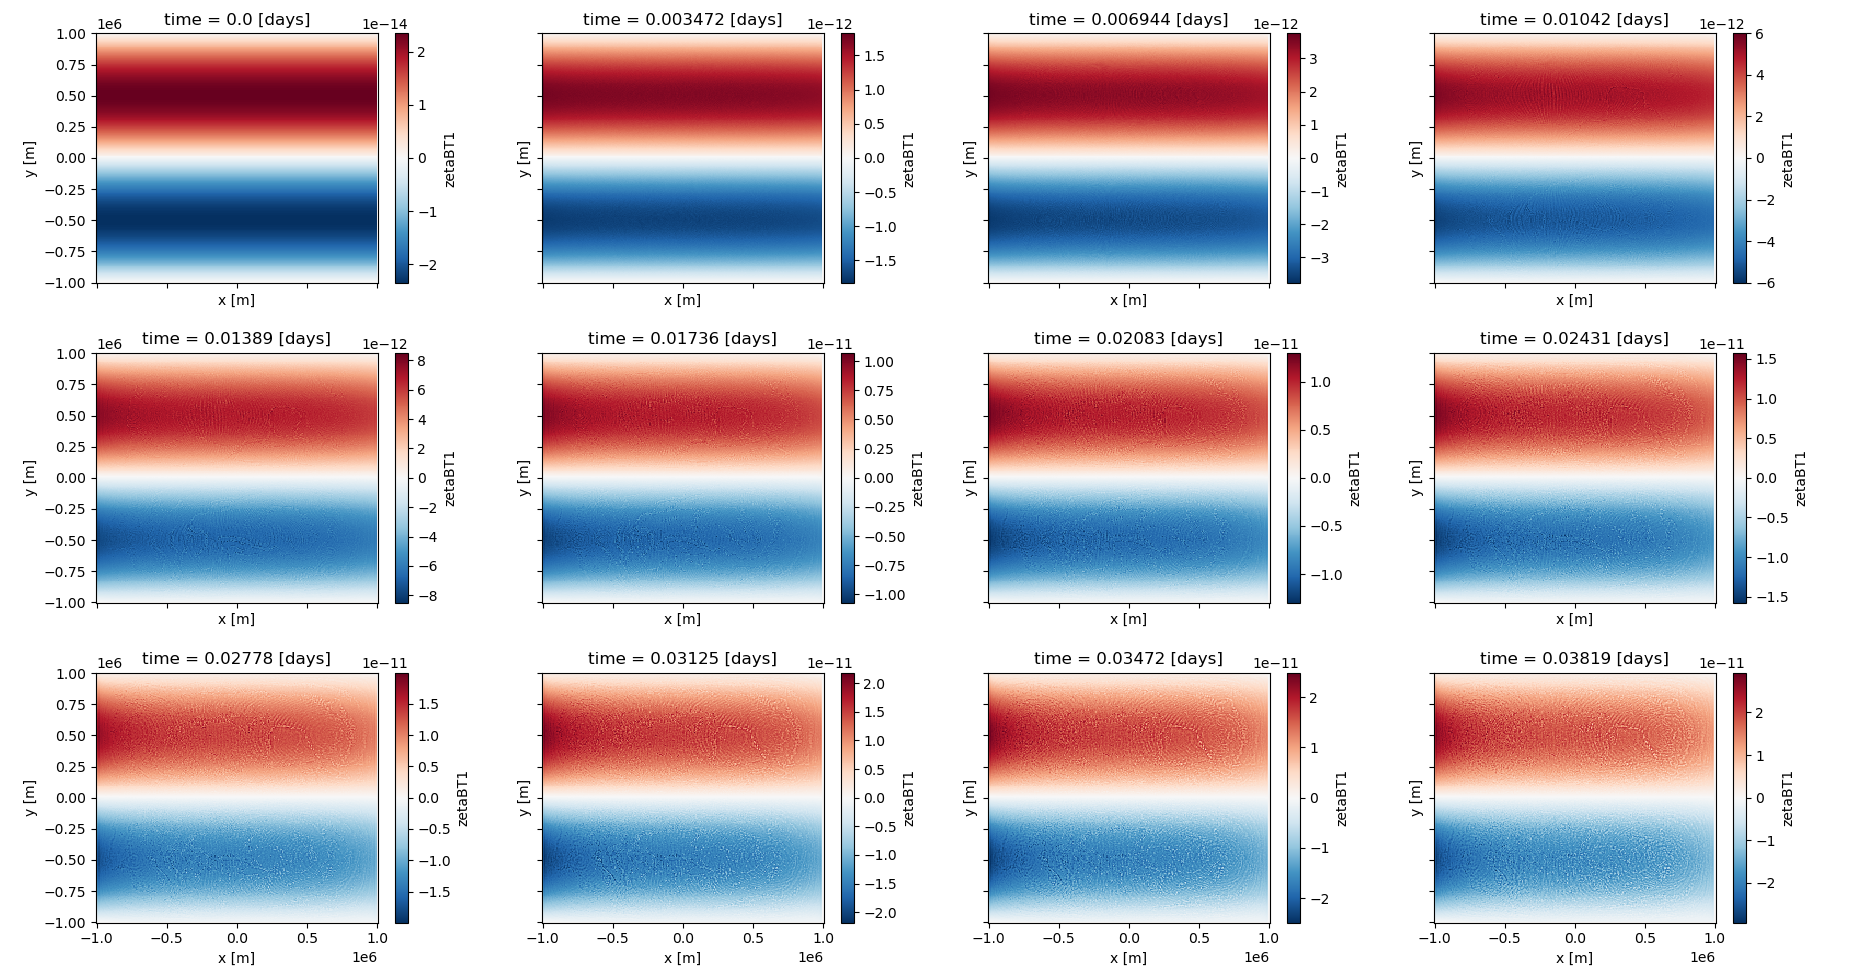
\includegraphics[width=.9\linewidth]{figures/debuggage/2023_08_23_zetaBT_4filesperdays.png}
\caption{\label{fig:org2384351}Test effectué dans le but d'obsever l'apparition des doubles gyres de Stommel (3 premiers jours).}
\end{figure}

\begin{figure}[htbp]
\centering
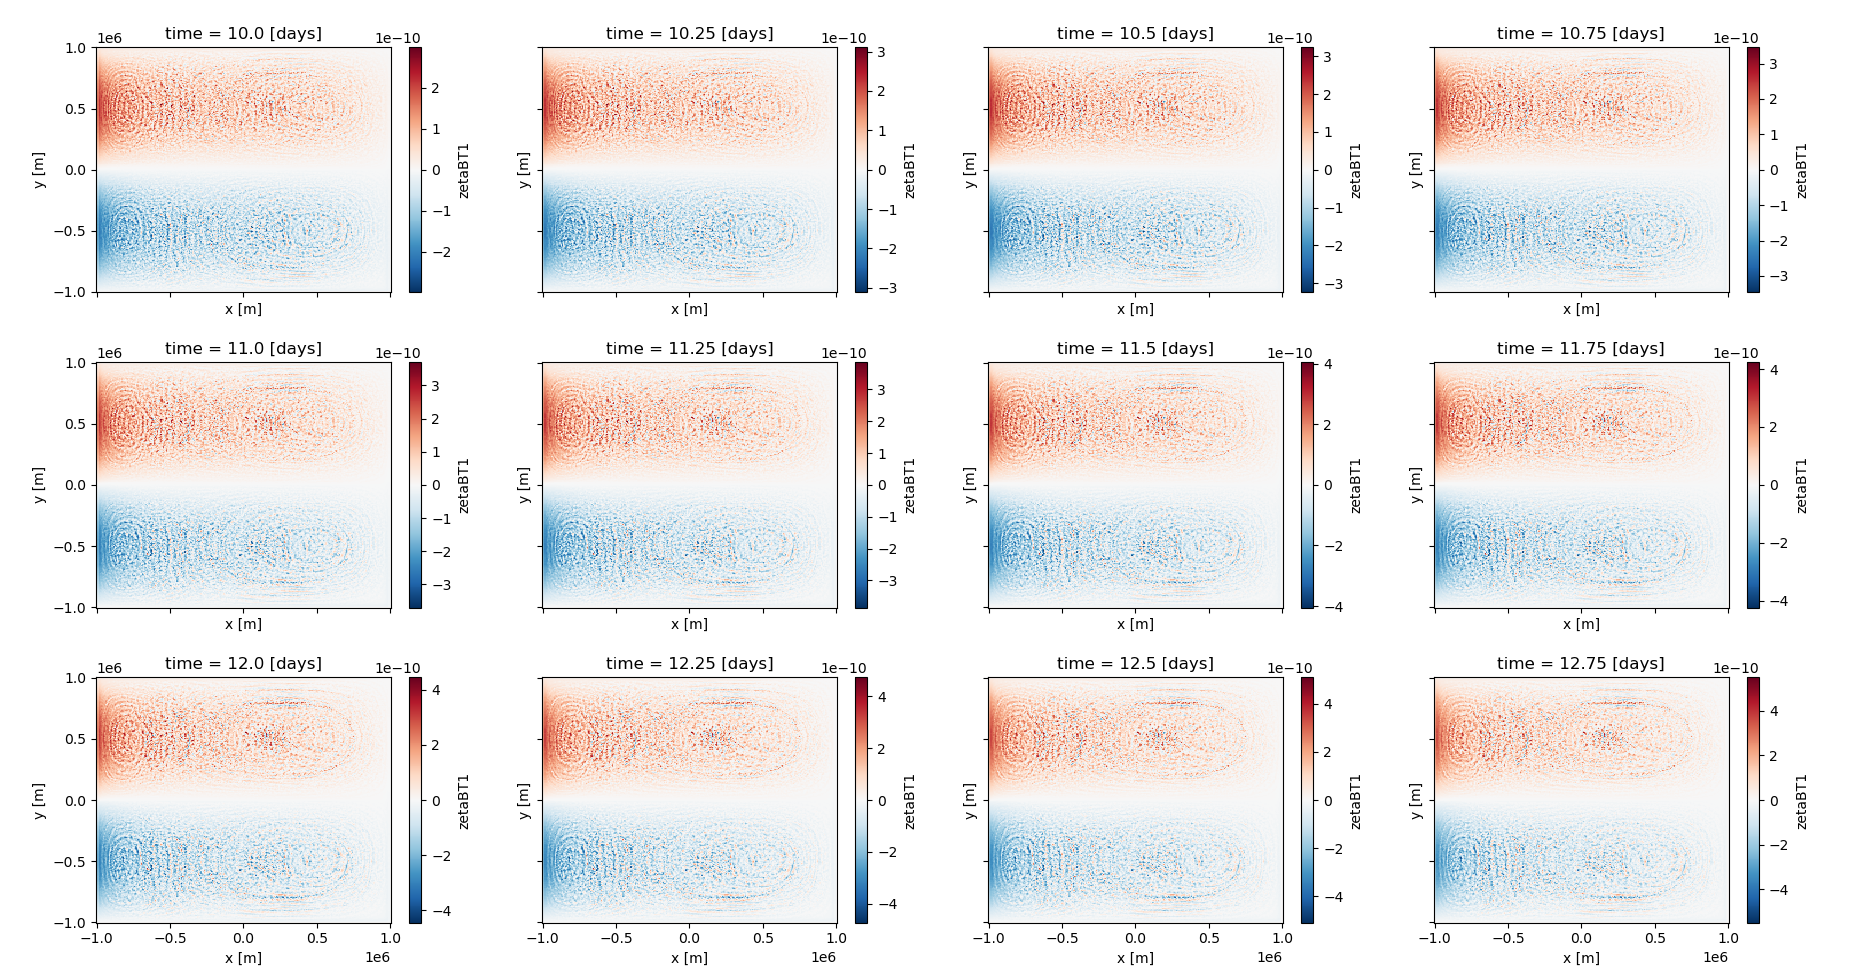
\includegraphics[width=.9\linewidth]{figures/debuggage/2023_08_23_zetaBT_4filesperdays2.png}
\caption{\label{fig:orge213f4e}Test effectué dans le but d'obsever l'apparition des doubles gyres de Stommel (10 à 12 jours).}
\end{figure}


\subsection{Provenance de l'erreur? -- \textit{<2023-08-18 Fri>}}
\label{sec:orgcfb563a}
D'où vient cette erreur?
Après un peu d'investigation, on voit que l'erreur se produit à cause des chiffres significatifs de \emph{MUDPACK} (Voir figure \ref{fig:org05ed9b5}).
La  méthode employée par \emph{MUDPACK} n'est pas suitable pour utiliser les chiffres de type \textbf{double precision}.
Il y a malheureusement trop de définitions de type \textbf{REAL} à l'intérieur de la fonction, elle-même.

\begin{figure}[htbp]
\centering
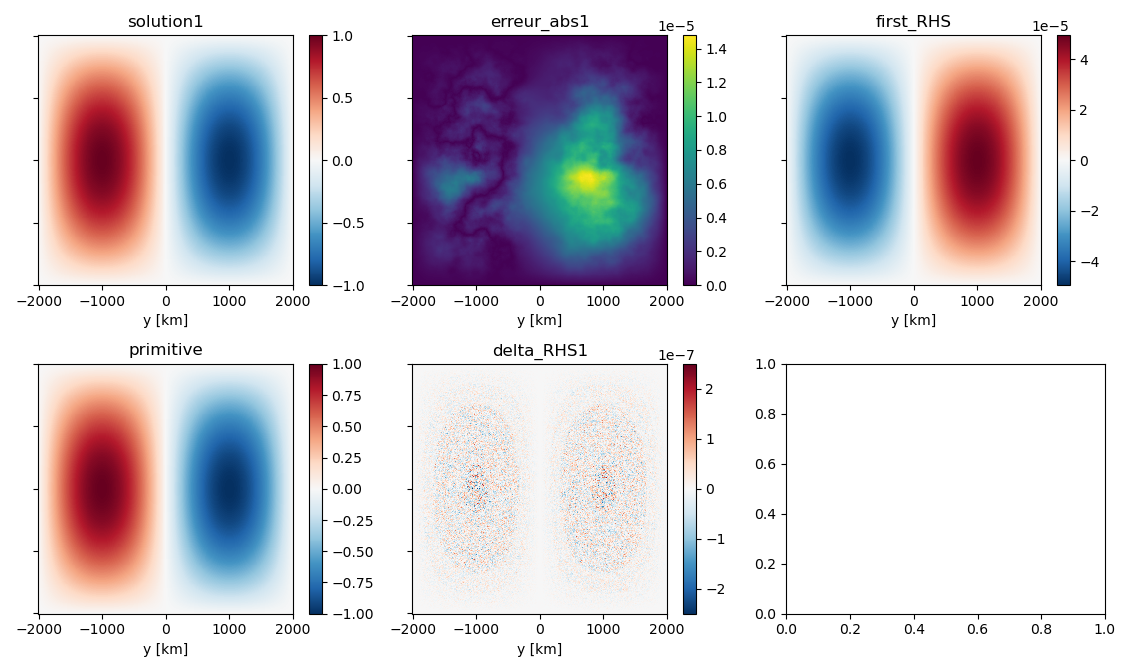
\includegraphics[width=.9\linewidth]{figures/MUDPACK/2023-08-23_MUDPACK_test_dirichlet.png}
\caption{\label{fig:org05ed9b5}Test de MUDPACK illustrant l'erreur issu lorsqu'on prend le laplacien de la solution trouvée.}
\end{figure}


\section{Limiter l'erreur de MUDPACK à l'aide de la proposition de David}
\label{sec:orgbc156c9}

\subsection{Explication de la méthode -- \textit{<2023-08-22 Tue>}}
\label{sec:orga646d0a}
\label{orgd7d7cfe}

Dans le modèle FFT, on appliquait la correction de pression deux fois pour s'assurer que la convergence était bonne.
L'idée de David Straub est essentiellement de faire la même chose, mais avec \emph{MUDPACK}, pour solidifier les solution qu'on trouve avec le module. \bigskip

En premier lieu, l'équation de Poisson à résoudre avec \emph{MUDPACK} est illustrée par
\begin{equation}
   \laplacian{\phi} = R_0,
\end{equation}
où \(n\) représente la \emph{profondeur} à laquelle nous appliquons les corrections.
\(\phi\) est la solution \emph{réelle} dont nous voulons nous approcher le plus possible.\bigskip

MUDPACK agit un peu comme la fonction inverse du Laplacien sur notre système d'équations, mais il n'est pas parfait, donc il induit de l'erreur dans la solution désirée.
La solution imparfaite trouvée avec \emph{MUDPACK} (soit \(\phi'\)) est représentée par 
\begin{align}
\label{eq:org6f9933e}
   && \phi' = MUD\qty[\pt R_0\pt\tall ], && \text{où} && \phi' = \phi + \delta\phi\pt(n=1).&&
\end{align}
Donc, la solution réelle est donnée par
\begin{equation}
\label{eq:org33a1baf}
   \phi = \phi' - \delta\phi(n=1).
\end{equation}
Rappellons que le \emph{prime} dénote que la solution n'est pas parfaite. En fait, comme illustré à droite de l'équation \ref{eq:org6f9933e}, la solution réelle est composée d'une solution imparfaite \(\phi'\) et d'une composante d'erreur ou d'un résidu \(\delta \phi(n=1)\).
Donc, si l'on trouve la valeur de la correction à appliquer (\(\delta\phi(n=1)\)), on devrait pouvoir trouver la solution réelle \(\phi\).\bigskip

Pour se faire, on applique le Laplacien sur l'équation \ref{eq:org33a1baf}, de sorte à obtenir
\begin{equation}
   \underbrace{\laplacian{\phi}}_{R_0} = \laplacian[\phi'] - \laplacian[\delta\phi(n=1)].
\end{equation}
Donc,
\begin{equation}
   \hspace{2mm} \underbrace{\laplacian[\delta\phi(1)]}_\text{Inconnu} = \laplacian[\phi'] - R_0 \equiv R(n=1).
\end{equation}

Et l'on repasse ça dans \emph{MUDPACK},
\begin{equation}
   \delta\phi'(1) = MUD\qty[\tall R(1) ],
\end{equation}


Bien entendu, comme on réutilise \emph{MUDPACK} pour résoudre notre équation différentielle partielle, on voit réapparaître des erreurs.
C'est pourquoi on utilise la notation \(\delta \tphi(1)\) pour dénoter l'approximation, de nouveau.
Au moins, l'erreur devrait être de plus en plus petite.
ce qui nous fait apparaître un nouveau second résidu \(\delta\phi(n=2)\), mais avec une erreur de plus en plus petite, ce qui se traduit par
\begin{equation}
   \delta\phi(1) > \delta\phi(2).
\end{equation}
On voit déjà où ça s'en va, mais continuons, comme dirait François Legault.
On veut connaître la valeur du second résidu, donc
\begin{equation}
   \delta \phi(2) = MUD\underbrace{\qty[R(1)\tall - \laplacian[\delta\phi(1)]]}_{R(2)}
\end{equation}
Donc, par définition
\begin{align}
   & R(n) \equiv R(n-1) - \laplacian[\delta\phi(n-1)\tall]\pt,\grande\\
   & \delta\phi(n) \equiv MUD\qty[R(n)\tall].\grande
\end{align}

Au final, on peut enchaîner les corrections jusqu'à être satisfait du résultat, soit
\begin{align}
   &\hspace{4mm}\phi(n) = \phi'(n) - \sum_n^\infty \delta\phi(n); \\
\end{align}

\subsection{Pas de cycles (Juste pour comparer)}
\label{sec:orgc74efa6}

Nous sortons cette figure seulement à titre de comparaison.

\begin{figure}[htbp]
\centering
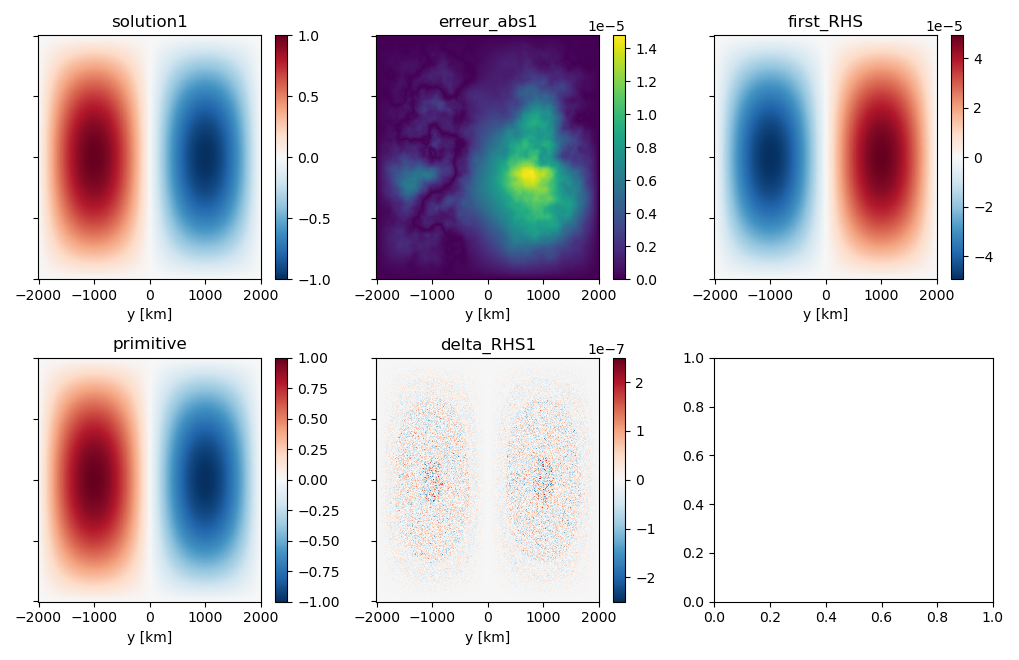
\includegraphics[width=.9\linewidth]{figures/MUDPACK/2023-08-23_MUDPACK_test_dirichlet0.png}
\caption{\label{fig:org52f8971}Différents champs d'intérêt pour tester MUDPACK après aucun cycle (pertinent pour comparer)}
\end{figure}


\subsection{Résultats de l'application de la méthode (Cycle 1) -- \textit{<2023-08-22 Tue>}}
\label{sec:org2564d53}
Si l'on applique un cycle supplémentaire avec la méthode de la section \ref{orgd7d7cfe}, on obtient des résultats intéressants.
Bref, on limite l'erreur d'environ 50\% (Voir figure \ref{fig:orgfc37f12}).

\begin{figure}[htbp]
\centering
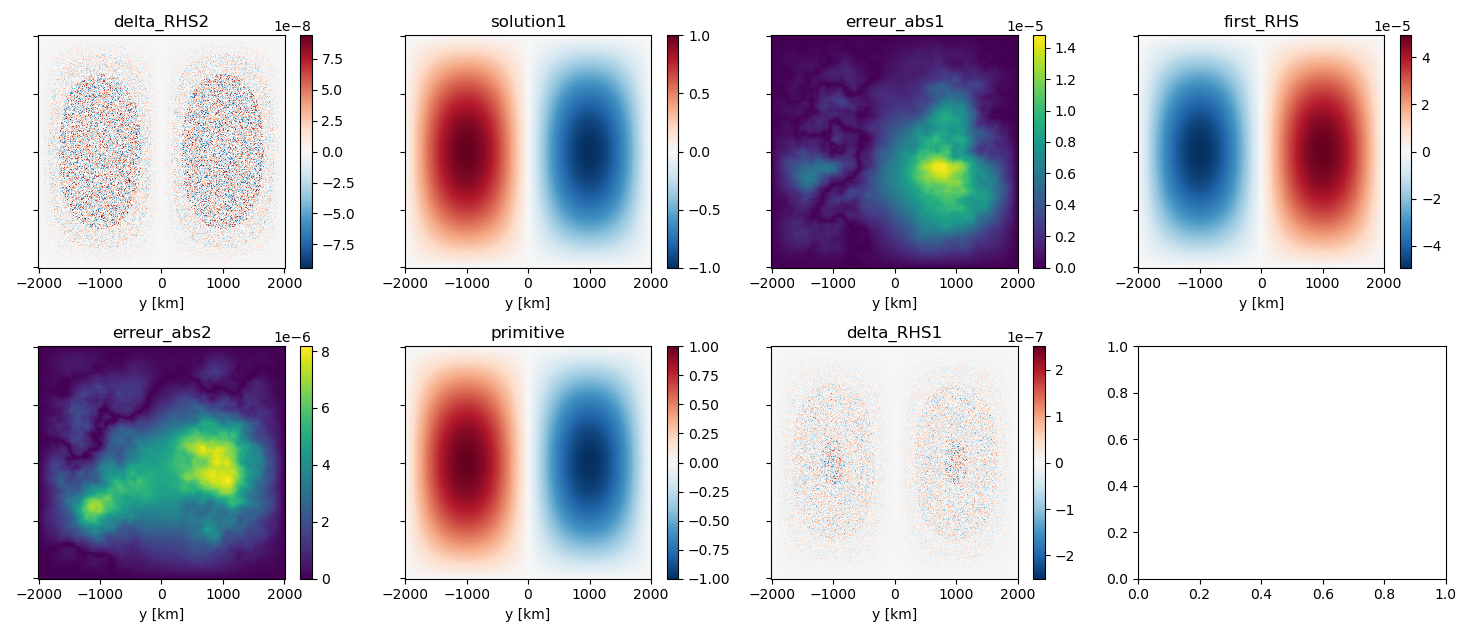
\includegraphics[width=.9\linewidth]{figures/MUDPACK/2023-08-23_MUDPACK_test_dirichlet2.png}
\caption{\label{fig:orgfc37f12}Différents champs d'intérêt pour tester MUDPACK après un seul cycles.}
\end{figure}

\subsection{Résultats de l'application de la méthode (Cycles > 1) -- \textit{<2023-08-24 Thu>}}
\label{sec:orge4143a5}
Voici un test avec deux cycles.
On observe que l'erreur associée à la précision de la solution diminue, mais pas l'erreur associée au Laplacien de la solution, illustrée à l'aide de la quantité \emph{delta RHS X} (Voir figure \ref{fig:org7a32230}).

\begin{figure}[htbp]
\centering
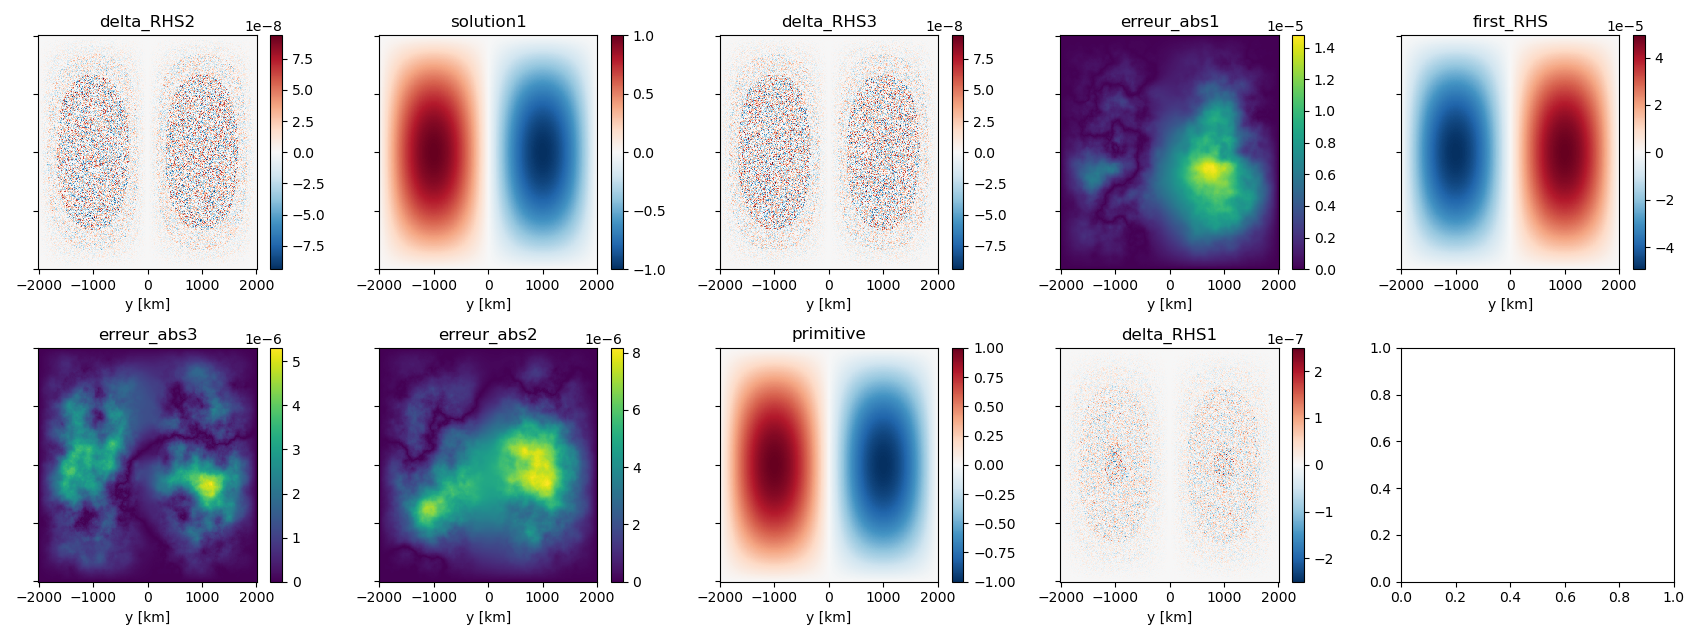
\includegraphics[width=.9\linewidth]{figures/MUDPACK/2023-08-23_MUDPACK_test_dirichlet3.png}
\caption{\label{fig:org7a32230}Différents champs d'intérêt pour tester MUDPACK après 2 cycles.}
\end{figure}

Un example éloquent de l'impact du problème sur nos résultats est aisément illustré par quelques « \emph{PRINT} » à l'intérieur du terminal pour comparer les écarts entre les cycles de \emph{MUDPACK} (Voir figure \ref{fig:org59ac378}).
\begin{itemize}
\item \emph{Max Abs Err} dénote le maximum de l'écart en valeur absolue entre la primitive et la solution approximée par MUDPACK,
\item \emph{MAXIMUM RHS} dénote le maximum associé au Laplacien de notre solution approximée par MUDPACK,
\item \emph{Max delta RHS} dénote l'écart entre les différents RHS trouvés.
\end{itemize}

\begin{figure}[!htpb]
\centering
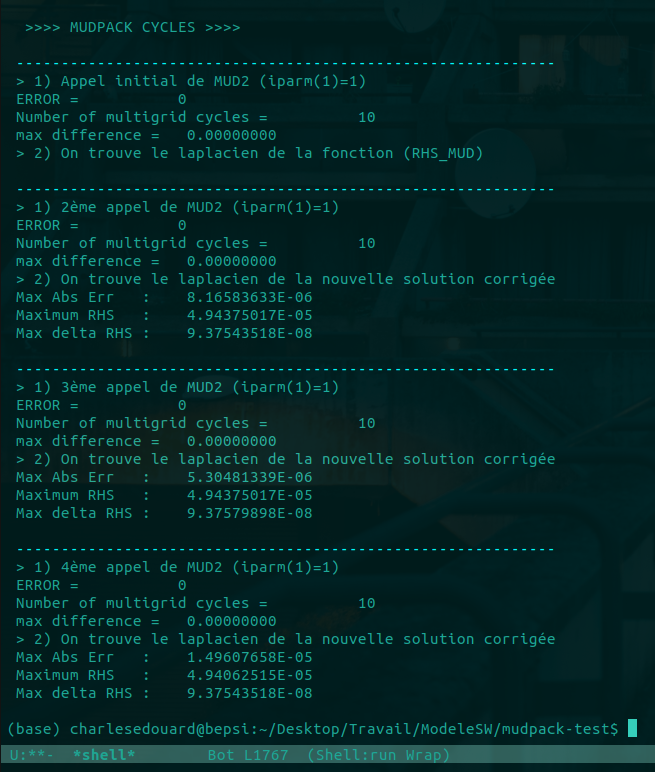
\includegraphics[width=\textwidth]{figures/debuggage/2023-08-28_screenshot.png}
\caption{\label{fig:org59ac378}Quantités intéressantes à sortir du terminal.}
\end{figure}
\end{document}